% XeLaTeX document
\documentclass[12pt,a4paper]{article}

% Редактируем: конфигурация, личные настройки: имя, название предмета и пр. для титульной страницы и метаданных документа здесь
\newcommand{\university}{Национальный исследовательский Университет ИТМО}
\newcommand{\mfaculty}{Мегафакультет информационных и трансляционных технологий}
\newcommand{\faculty}{Факультет инфокоммуникационных технологий}
\newcommand{\city}{Санкт-Петербург}
\newcommand{\num}{ №1}
\newcommand{\docname}{Лабораторная работа}
\newcommand{\subject}{Инфокоммуникационные системы и технологии}
\newcommand{\tutorname}{О.М. Ромакина}
\newcommand{\studentname}{К.М. Долгов}
\newcommand{\group}{К3122}

% Не редактируем: используемые пакеты
% настройка кодировки, шрифтов и русского языка
\usepackage{fontspec}
\usepackage{polyglossia}

% рабочие ссылки в документе
\usepackage{hyperref}

% графика
\usepackage{graphicx}
\usepackage{tikz}

% поворот страницы
\usepackage{pdflscape}

% качественные листинги кода
\usepackage{minted}
\usepackage{listings}
\usepackage{lstfiracode}

% отключение копирования номеров строк из листинга, работает не во всех просмотрщиках (в Adobe Reader работает)
\usepackage{accsupp}
\newcommand\emptyaccsupp[1]{\BeginAccSupp{ActualText={}}#1\EndAccSupp{}}
\let\theHFancyVerbLine\theFancyVerbLine
\def\theFancyVerbLine{\rmfamily\tiny\emptyaccsupp{\arabic{FancyVerbLine}}}

% библиография
\bibliographystyle{templates/gost-numeric.bbx}
\usepackage{csquotes}
\usepackage[parentracker=true,backend=biber,hyperref=true,bibencoding=utf8,style=numeric-comp,language=auto,autolang=other,citestyle=gost-numeric,defernumbers=true,bibstyle=gost-numeric,sorting=ntvy]{biblatex}

% установка полей
\usepackage{geometry}

% нумерация картинок по секциям
\usepackage{chngcntr}

% дополнительные команды для таблиц
\usepackage{booktabs}

% для заголовков
\usepackage{caption}
\usepackage{titlesec}
\usepackage[dotinlabels]{titletoc}

% разное для математики
\usepackage{amsmath, amsfonts, amssymb, amsthm, mathtools}

% водяной знак на документе, см. main.tex
\usepackage[printwatermark]{xwatermark}

% Не редактируем: параметры используемых пакетов и не только
% настройки polyglossia
\setdefaultlanguage{russian}
\setotherlanguage{english}

% локализация
\addto\captionsrussian{
	\renewcommand{\figurename}{Рисунок}%
	\renewcommand{\partname}{Глава}
	\renewcommand{\contentsname}{\centerline{Содержание}}
	\renewcommand{\listingscaption}{Листинг}
}

% основной шрифт документа
\setmainfont{CMU Serif}
\newfontfamily\cyrillicfont{CMU Serif}[Script=Cyrillic]

% перечень использованных источников
\addbibresource{refs.bib}

% настройка полей
\geometry{top=2cm}
\geometry{bottom=2cm}
\geometry{left=2cm}
\geometry{right=2cm}
\geometry{bindingoffset=0cm}

% настройка ссылок и метаданных документа
\hypersetup{unicode=true,colorlinks=true,linkcolor=red,citecolor=green,filecolor=magenta,urlcolor=cyan,
	pdftitle={\docname},
	pdfauthor={\studentname},
	pdfsubject={\subject},
	pdfcreator={\studentname},
	pdfproducer={Overleaf},
	pdfkeywords={\subject}
}

% настройка подсветки кода и окружения для листингов
\usemintedstyle{colorful}
\newenvironment{code}{\captionsetup{type=listing}}{}

% шрифт для листингов с лигатурами
\setmonofont{FiraCode-Regular.otf}[
	SizeFeatures={Size=10},
	Path = templates/,
	Contextuals=Alternate
]

% оформления подписи рисунка
\captionsetup[figure]{labelsep = period}

% подпись таблицы
\DeclareCaptionFormat{hfillstart}{\hfill#1#2#3\par}
\captionsetup[table]{format=hfillstart,labelsep=newline,justification=centering,skip=-10pt,textfont=bf}

% путь к каталогу с рисунками
\graphicspath{{fig/}}

% Внесение titlepage в учёт счётчика страниц
\makeatletter
\renewenvironment{titlepage} {
	\thispagestyle{empty}
}
\makeatother

\counterwithin{figure}{section}
\counterwithin{table}{section}

\titlelabel{\thetitle.\quad}

% для удобного конспектирования математики
\mathtoolsset{showonlyrefs=true}
\theoremstyle{plain}
\newtheorem{theorem}{Теорема}[section]
\newtheorem{proposition}[theorem]{Утверждение}
\theoremstyle{definition}
\newtheorem{corollary}{Следствие}[theorem]
\newtheorem{problem}{Задача}[section]
\theoremstyle{remark}
\newtheorem*{nonum}{Решение}

% настоящее матожидание
\newcommand{\MExpect}{\mathsf{M}}

% объявили оператор!
\DeclareMathOperator{\sgn}{\mathop{sgn}}

% перенос знаков в формулах (по Львовскому)
\newcommand*{\hm}[1]{#1\nobreak\discretionary{} {\hbox{$\mathsurround=0pt #1$}}{}}


% водяной знак для обозначения статуса документа
%\newwatermark[allpages,color=red!5,angle=45,scale=3,xpos=0,ypos=0]{DRAFT}
\begin{document}
% Не редактируем: Титульная страница (формируется автоматически из заданной конфигурации)
\begin{titlepage}	% начало титульной страницы

	\begin{center}		% выравнивание по центру

		\large \university \\
		\large \mfaculty \\
		\large \faculty \\[6cm]
		% название института, затем отступ 6см

		\huge \subject \\[0.5cm] % название работы, затем отступ 0,5см
		\large \docname  \num \\[5.1cm]
		 %\large Разработка методов обучения с подкреплением\\[5cm]

	\end{center}


	\begin{flushright} % выравнивание по правому краю
		\begin{minipage}{0.25\textwidth} % врезка в половину ширины текста
			\begin{flushleft} % выровнять её содержимое по левому краю

				\large\textbf{Работу выполнил:}\\
				\large \studentname \\
				\large {Группа:} \group \\

				\large \textbf{Преподаватель:}\\
				\large \tutorname

			\end{flushleft}
		\end{minipage}
	\end{flushright}

	\vfill % заполнить всё доступное ниже пространство

	\begin{center}
		\large \city \\
		\large \the\year % вывести дату
	\end{center} % закончить выравнивание по центру

\end{titlepage} % конец титульной страницы

\vfill % заполнить всё доступное ниже пространство


% Не редактируем: Страница содержания (формируется автоматически из section, subsection и пр., указанных в content.tex)
% Содержание
\tableofcontents
\newpage



% Редактируем: всё остальное: вступление, др. этапы, заключение, приложение
\section*{Введение}
Практическая работа посвящена оформлению математического текста с формулами и рисунками, а также оформлению таблицы с профессиями при помощи системы верстки LaTeX.

Цель работы: оформить 3 страницы математического текста и таблицу с профессиями согласно правилам оформления ГОСТ 7.32.

\addcontentsline{toc}{section}{Введение}

\newpage
\section{Определение и необходимые условия экстремума функции нескольких переменных}
\textbf{Определение 1.1} Пусть функция
\[ f(x) = f(x_1,x_2,...,x_n) \]
определена в некоторой окрестности точки

\[  x_0 = (x_0^1,x_0^2,...,x_0^n). \]

Говорят, что функция $f(x)$ имеет в точке $x_0$ \textit{локальный максимум (минимум)}, если существует такая окрестность точки $x_0$, в которой для всех $x \neq x_0$ выполняется неравенство \eqref{formula}
\begin{equation}\label{formula}
    f(x) \leq f(x0) (f(x) \geq f(x0))
\end{equation}
Если для всех $x \neq x_0$ из некоторой окрестности точки $x_0$
выполняется строгое неравенство
\[f(x) < f(x0) (f(x) > f(x0)),\]
то $x_0$ называются \texit{точкой строгого максимума (минимума)} функции.

Точки максимума и минимума функции называются \textit{точками экстремума}, а значения функции в этих точках называется \texit{экстремумами функции}.

\textbf{Теорема 1.1} (необходимое условие экстремума). 
\textit{Если точка $(x^0_1, x^0_2, . . . , x^0_n)$ является точкой экстремума функции $f(x_1, x_2, . . . , x_n)$ и в этой точке существует частная производная $\frac{\partial f}{\partial x_i}(x_0),$ то она равна нулю.}

\textit{Доказательство.} Рассмотрим функцию одной переменной $x_i$:
\[g(x_i) = f(x^0_1,...,x^0_i−1,x_i,x^0_i+1,...,x^0_n).\]

Существование конечной частной производной функции
$f(x_1 , . . . , x_n )$ по переменной $xi_$ в точке $x_0$ эквивалентно
дифференцируемости функции $g(x_i)$ в точке $x^0_i$ . Очевидно,
что функцияg ($x_i$) имеет в точке $x^0_i$ локальный экстремум.
А тогда $g'(x^0_i ) = 0.$ Это означает, что $f'_x_i (x_0) = 0.$ Теорема доказана.

Если функция $f(x_1, x_2, . . . , x_n)$ имеет в точке $x_0$ локальный экстремум и дифференцируема в этой точке, то частные производные по всем переменным в этой точке равны нулю (формула \eqref{formula:2}):

\begin{equation}
    \label{formula:2}
    \frac{\partial f}{\partial x_1} = 0, \frac{\partial f}{\partial x_2} = 0, . . . \frac{\partial f}{\partial x_n} = 0\
\end{equation}
    
а следовательно,
\[df(x^0_1, x^0_2, . . . , x^0_n) = 0. \]
Точки, координаты которых удовлетворяют системе уравнений (1.2), называют \textit{точками, подозрительными на экстремум (или стационарными точками)}. Точки экстремума функции следует искать только среди точек, подозрительных на экстремум.

Оказывается, не любая стационарная точка является точкой локального экстремума дифференцируемой функции. Например, для функции $f(x, y) = x^2 + y^2$ (рис. 1.1) точка (0; 0) является и стационарной:

\[df(0,0)=2xdx+2ydy|_{(0,0)} = 0,\]
и точкой локального минимума:
\[f(x,y)=x^2 +y^2 \geq 0=f(0,0),\]
а для функции $f (x, y) = x^2 − y^2$ (рис. 18.2) точка (0; 0)
является стационарной:
\[df(0,0)=2xdx-2ydy|_{(0,0)} = 0,\]
но не является точкой локального экстремума, так как в любой окрестности точки (0; 0) функция принимает и положительные и отрицательные значения:
\[f(\varepsilon, 0) = \varepsilon^2, f(0, \varepsilon) = −\varepsilon^2.\]

\begin{center}
\begin{tabular}{ c c } 
 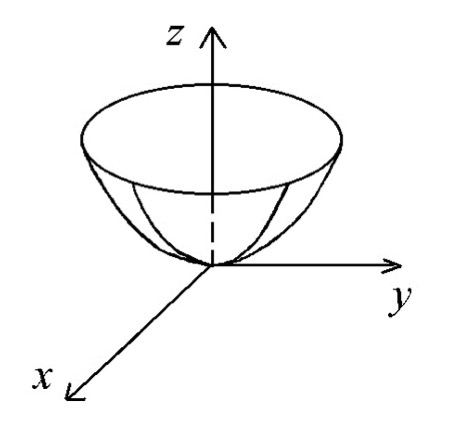
\includegraphics[width=.4\textwidth]{pic_1.jpg} & 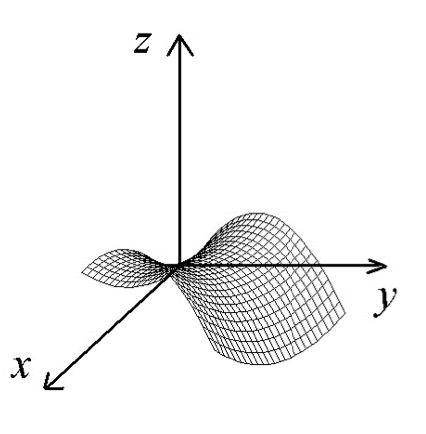
\includegraphics[width=.4\textwidth]{pic_2.jpg}\\
 Рисунок 1.1 - Полусфера & Риуснок 1.2 - Волна
\end{tabular}
\end{center}

Следовательно, для исследования локального экстремума нужны некоторые достаточные условия.

Предварительно вспомним алгебраические понятия. \cite{litlink1}


\begin{table}[H]
	\caption{График защиты курсовой работы}
	\begin{center}
		\begin{tabular*}{0.4\textwidth}{@{\extracolsep{\fill} } lcc}
			\toprule
			Дата & 12:00 & 17:00 \\
			\midrule
			20.12       & Долгов К.   & Калинин А.   \\
			23.12       & Суслопаров В.    & Волкович К.    \\
			25.12     & Сергеев А.   & Теребов М.   \\
			27.12      & Шестаков М.   & Драчева Е.    \\
			\bottomrule
		\end{tabular*}
		\label{tabular:tab_examp_1}
	\end{center}
\end{table}


\newpage
\section*{Заключение}

Цель работы достигнута: в ходе работы были оформлены  3 страницы математического текста с формулами и рисунками и таблица с профессиями согласно стандартам оформления. Данная работа помогла ознакомится с инструментами системы компьютерной верстки LaTeX.

\addcontentsline{toc}{section}{Заключение}

% Не редактируем: Страница библиографии (формируется автоматически из книжек, указанных в refs.bib и пометок \cite{имя_источника} в тексте)
\newpage
\printbibliography[title=Список использованных источников]
\addcontentsline{toc}{section}{Список использованных источников}
\end{document}
